\section{Introduzione}
    \begin{definition}[Rete]
        Un’interconnessione di dispositivi in grado di scambiarsi
        informazioni, quali sistemi terminali (host), router, switch e modem
    \end{definition} 

    \begin{definition}[Router]
        Dispositivi che interconnettono reti.
    \end{definition} 

    \begin{definition}[Switch]
        Dispositivi che collegano fra loro più host a livello locale
    \end{definition}

    \paragraph*{Tipologie di reti} Esistono varie tipologie di reti
        \begin{itemize}
            \item \textbf{\textcolor{purple}{LAN}}: Local Area Network, sono reti di piccole dimensioni (al più qualche km). Connettono principalmente host, stampanti e workstation tra loro.
            \item \textbf{\textcolor{purple}{WAN}}: Wide Area Network, è una rete il cui compito è di interconnettere LAN o singoli host separati da distanze geografiche.
            \item \textbf{\textcolor{purple}{MAN}}: Metropolitan Area Network, rete di computer che collega i computer all'interno di un'area metropolitana, più grande di una LAN ma più piccola di una WAN.
        \end{itemize}

    \paragraph*{Network of networks} Gli host si collegano ad internet tramite Internet Service Provider (ISP) i quali devono a loro volta essere connessi tra loro. La risultante rete di reti è molto complessa.
    \begin{figure}[h]
        \centering
        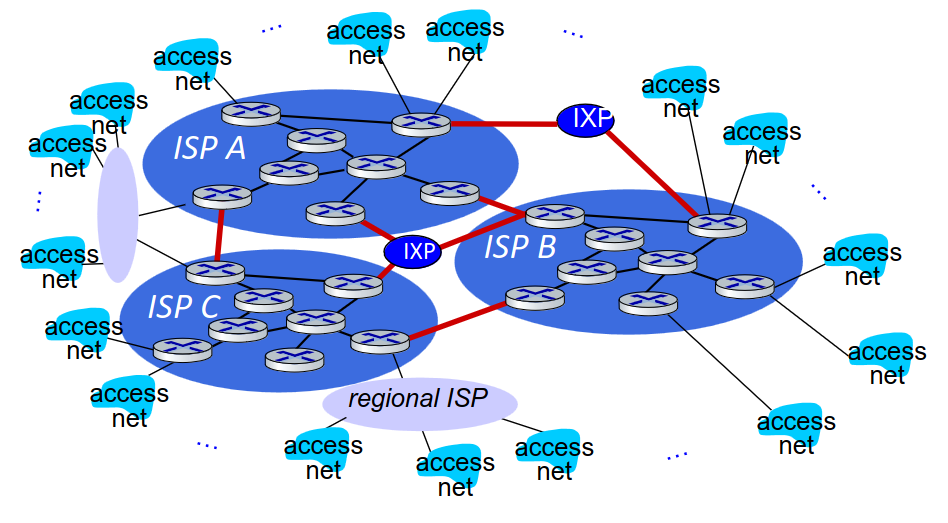
\includegraphics[scale=0.35]{Immagini/Rete-di-Reti.png}
        \caption{Struttura della rete Internet}
    \end{figure}
    